\documentclass[a4paper,oneside,11pt]{book}

% Format utama mengikuti template laporan Praktikum Pertemuan 6
\usepackage[utf8]{inputenc}
\usepackage[T1]{fontenc}
\usepackage{graphicx}
\usepackage{titling}
\usepackage[indonesian]{babel}
\usepackage{titlesec}
\usepackage{geometry}
\usepackage{setspace}
\usepackage{fancyhdr}
\usepackage{hyperref}
\usepackage{listings}
\usepackage{xcolor}
\usepackage{float}
\usepackage{tocloft}
\usepackage{indentfirst}
\geometry{left=3cm,right=2cm,top=2cm,bottom=2cm}
\setlength{\headheight}{14pt}
\onehalfspacing

\titleformat{\chapter}[hang]
  {\normalfont\huge\bfseries\centering}{\chaptertitlename\ \thechapter.}{1em}{}
\titleformat{\section}[hang]
  {\normalfont\Large\bfseries}{\thesection}{1em}{}
\titleformat{\subsection}[hang]
  {\normalfont\Large\bfseries}{\thesubsection}{1em}{}
\titleformat{\subsubsection}[hang]
  {\normalfont\large\bfseries}{\thesubsubsection}{1em}{}
\titlespacing*{\section}{0pt}{1.5ex}{1ex}
\titlespacing*{\subsection}{0pt}{1.3ex}{0.8ex}
\titlespacing*{\subsubsection}{0pt}{1.2ex}{0.7ex}

\lstdefinelanguage{PHP}{
  morekeywords={abstract,and,array,as,break,callable,case,catch,class,clone,const,continue,declare,default,do,echo,else,elseif,empty,endfor,endforeach,endif,endswitch,endwhile,extends,final,finally,for,foreach,function,global,if,implements,include,instanceof,interface,namespace,new,null,or,print,private,protected,public,require,return,static,switch,throw,trait,try,use,var,while,yield,true,false},
  sensitive=true,
  morecomment=[l]{//},
  morecomment=[s]{/*}{*/},
  morestring=[b]',
  morestring=[b]"
}
\lstset{
  basicstyle=\ttfamily\scriptsize,
  keywordstyle=\color{blue!65!black},
  commentstyle=\color{gray!75!black},
  stringstyle=\color{red!55!black},
  numbers=left,
  numberstyle=\tiny\color{gray},
  frame=single,
  breaklines=true,
  breakatwhitespace=false,
  showstringspaces=false,
  keepspaces=true,
  columns=fullflexible,
  tabsize=4,
  xleftmargin=1em,
  framexleftmargin=1em,
  captionpos=b
}
\hypersetup{colorlinks=true,linkcolor=black,urlcolor=blue,citecolor=red,hypertexnames=false}

\title{Laporan Praktikum \\
Pemrograman Web 2\\
Pertemuan 6\\
Seeder, Query Data, Filter, Statistik, dan Pencarian}
\author{Nama Mahasiswa: Reyhan Abelard Fikri\\NIM: 25/56200/SV/26713}

\begin{document}
% Title Page
\begin{titlingpage} 
\begin{center}

\vspace{4cm} 
\begin{Large} 
\textbf{\thetitle} \\
\end{Large}
\vspace{2cm}


\includegraphics[height=8cm]{lambang ugm.png}\\ 
\begin{large}
\vspace{2cm} 
\theauthor\\
Kelas: A1 \\ 
\end{large}
\begin{large}
Dosen Pengampu: Dinar Nugroho Pratomo, S.Kom., M.IM., M.Cs.\\
\end{large}

\vspace{2cm}
\begin{Large}
\textbf{Sekolah Vokasi}\\
\textbf{Universitas Gadjah Mada}\\
\textbf{Yogyakarta}\\
\textbf{2026}\\
\end{Large}

\end{center}
\end{titlingpage}

\pagestyle{fancy}
\fancyhf{}
\fancyhead[L]{Laporan Praktikum}
\fancyhead[R]{Praktikum Pemrograman Web 2}
\fancyfoot[C]{\thepage}

\setcounter{tocdepth}{3}
\setcounter{secnumdepth}{3}
\renewcommand{\cfttoctitlefont}{\hfill\normalfont\huge\bfseries}
\renewcommand{\cftaftertoctitle}{\hfill}
\renewcommand{\cftbeforetoctitleskip}{0pt}
\renewcommand{\cftaftertoctitleskip}{20pt}
\renewcommand{\cftchappresnum}{Bab }
\renewcommand{\cftchapaftersnum}{.}
\renewcommand{\cftchapnumwidth}{3.7em}
\tableofcontents
\clearpage

\chapter{Pendahuluan}
\section{Latar Belakang}
Pengelolaan data merupakan bagian penting dalam pengembangan aplikasi web. Pada praktikum ini, fitur pengelolaan data diterapkan pada dua proyek Laravel, yaitu katalog buku dan daftar event lari. Data awal disiapkan menggunakan seeder, kemudian ditampilkan dan diolah melalui controller serta view Blade.

\section{Tujuan Praktikum}
\begin{enumerate}
  \item Membuat data awal menggunakan seeder dengan 20 record pada masing-masing proyek.
  \item Menampilkan lima data terbaru pada halaman web.
  \item Menerapkan penyaringan data berdasarkan penulis atau tipe event.
  \item Menampilkan statistik yang sesuai dengan data proyek.
  \item Menerapkan pencarian serta memberikan informasi ketika hasil tidak ditemukan.
\end{enumerate}

\chapter{Dasar Teori}
\section{Seeder dan Data Awal}
Seeder adalah kelas Laravel yang digunakan untuk mengisi basis data dengan data awal. Method \texttt{run()} pada seeder memuat operasi penyimpanan data, sedangkan \texttt{DatabaseSeeder} dapat memanggil seeder lain untuk mengatur rangkaian pengisian data. Pada proyek ini, data buku dan event didefinisikan pada seeder masing-masing.\cite{laravel-seeding}

\section{Model, Controller, dan Routing}
Model mewakili data yang disimpan di basis data. Controller menerima permintaan, menjalankan query melalui model, dan mengirimkan data yang diperlukan ke view. Route menghubungkan alamat URL dengan method controller sehingga halaman dapat dibuka melalui browser.\cite{laravel-routing}

\section{View Blade}
Blade merupakan template engine Laravel yang menyediakan sintaks untuk menampilkan data, melakukan perulangan, dan memilih tampilan berdasarkan kondisi. Dalam proyek ini, view menampilkan tabel, formulir GET, pesan hasil kosong, serta statistik.\cite{laravel-blade}

\section{Filter, Pencarian, dan Statistik}
Filter memilih record yang sesuai dengan nilai tertentu, misalnya penulis atau tipe event. Pencarian membandingkan kata kunci dengan judul buku atau nama event. Statistik dapat dihitung dari data menggunakan operasi hitung seperti jumlah, total, nilai maksimum, dan nilai minimum. Laravel menyediakan query dan koleksi untuk membantu proses pemilihan serta pengolahan data.\cite{laravel-query}

\chapter{Hasil dan Pembahasan}
Praktikum dibahas melalui dua proyek. Kode yang ditampilkan pada subbab berikut disalin dari berkas proyek, sedangkan gambar merupakan bukti tampilan web pada saat fitur dijalankan.

\section{Proyek Buku}
Proyek Buku menggunakan tabel \texttt{books} dengan atribut judul, penulis, harga, dan tanggal terbit. Seeder mengisi 20 data. Controller menyajikan lima data terbaru, hasil filter atau pencarian, serta statistik. Route halaman buku menggunakan alamat \texttt{/buku}.

\subsection{Struktur Model dan Seeder Buku}
Model \texttt{Buku} menghubungkan aplikasi dengan tabel \texttt{books}. Seeder berisi 20 record yang dimasukkan menggunakan model.
\lstinputlisting[language=PHP,caption={Model Buku}]{Kode/Buku.php}
\lstinputlisting[language=PHP,caption={Seeder berisi 20 data buku}]{Kode/BukuSeeder.php}

\subsection{Controller Buku}
Method \texttt{index()} mengambil lima buku terbaru, menerima parameter penulis dan kata kunci, menerapkan filter, lalu menghitung statistik dari hasil data yang akan ditampilkan.
\lstinputlisting[language=PHP,caption={Logika daftar, filter, pencarian, dan statistik buku}]{Kode/BukuController.php}

\subsection{Route dan View Buku}
Route menghubungkan URL \texttt{/buku} ke \texttt{BukuController}. View menampilkan tabel buku, dropdown penulis, form pencarian, pesan hasil kosong, dan nilai statistik dalam format Rupiah.
\begin{lstlisting}[language=PHP,caption={Route halaman buku}]
Route::get('/buku', [BukuController::class, 'index'])
    ->name('buku.index');
\end{lstlisting}
\lstinputlisting[caption={View halaman Data Buku}]{Kode/buku.blade.php}

\subsection{Hasil Halaman Buku}
Pada tampilan awal, halaman menampilkan lima buku terbaru serta seluruh 20 data buku. Statistik awal menunjukkan total harga Rp 1.400.000, harga tertinggi Rp 100.000, dan harga terendah Rp 40.000.
\begin{figure}[H]
  \centering
  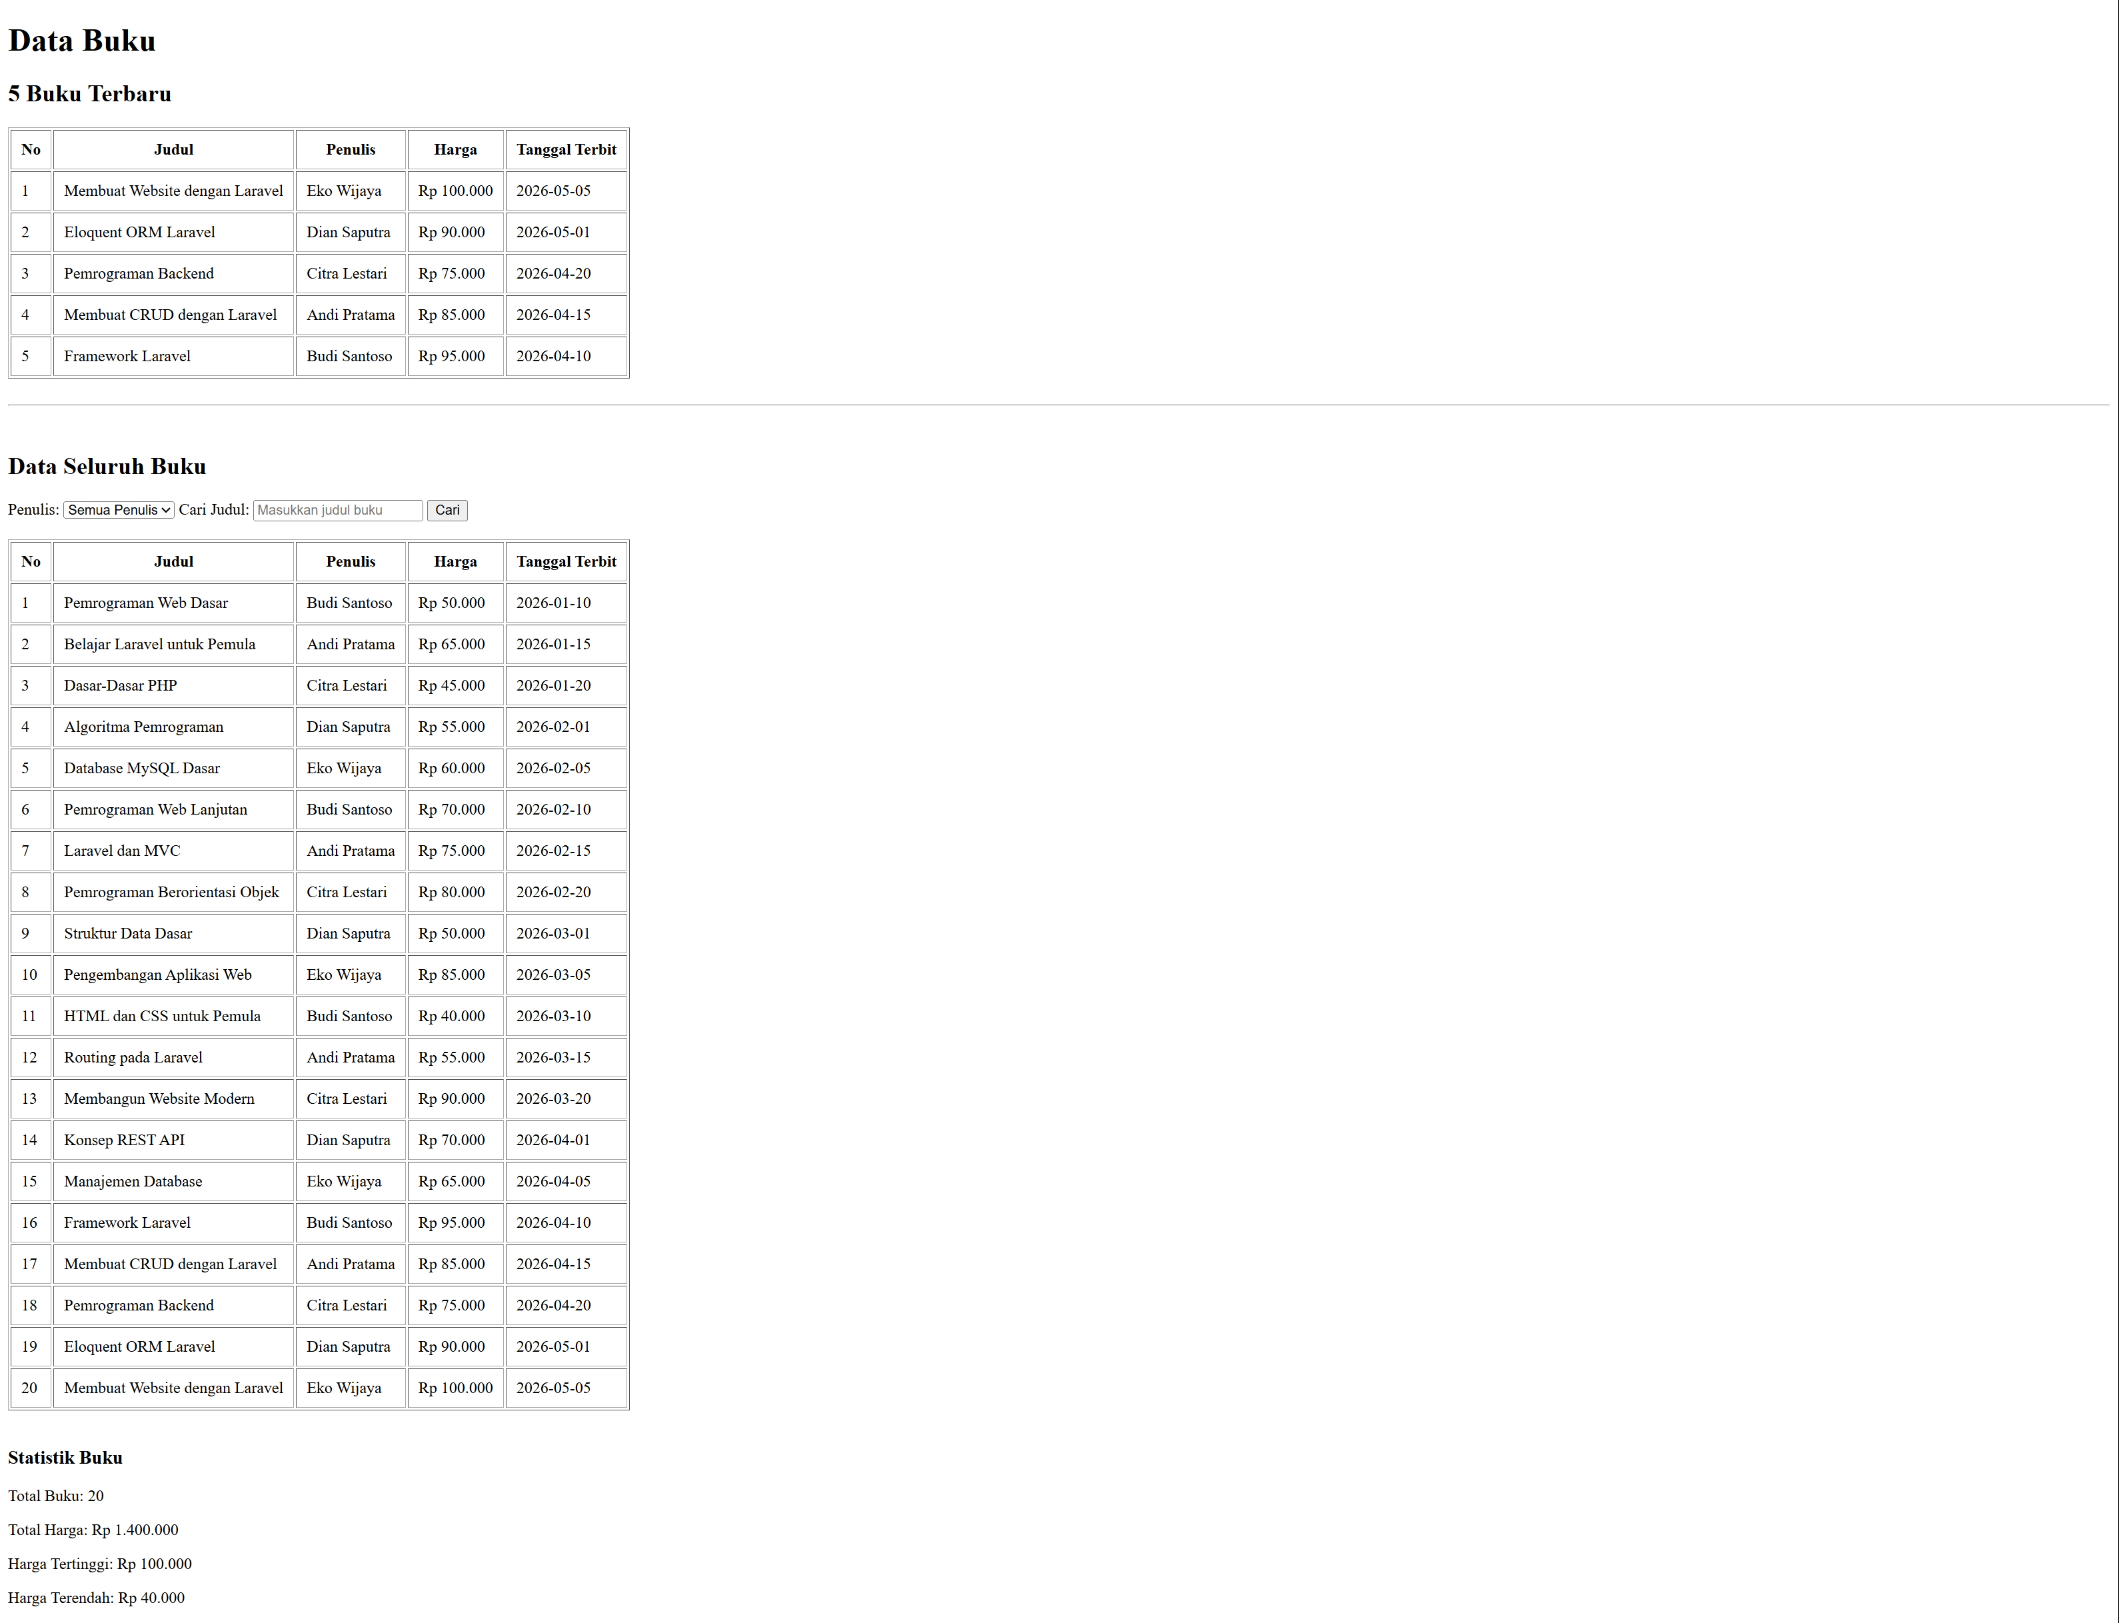
\includegraphics[height=0.72\textheight,keepaspectratio,trim=0bp 0bp 1300bp 0bp,clip]{Screenshot/buku-full-page.png}
  \caption{Tampilan lengkap halaman Buku, termasuk lima data terbaru, 20 buku, dan statistik.}
\end{figure}

\subsection{Filter Berdasarkan Penulis}
Dropdown penulis digunakan untuk menampilkan buku dari penulis yang dipilih. Contoh berikut menunjukkan hasil filter untuk Budi Santoso.
\begin{figure}[H]
  \centering
  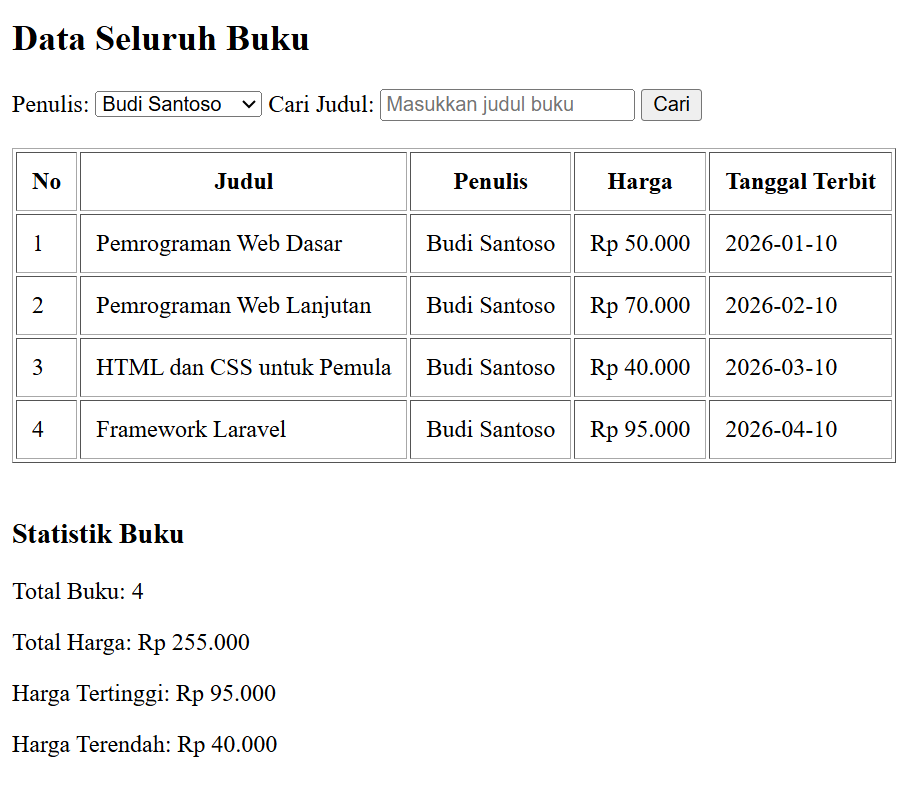
\includegraphics[width=0.96\textwidth,height=0.58\textheight,keepaspectratio]{Screenshot/buku-filter.png}
  \caption{Hasil filter buku berdasarkan penulis Budi Santoso.}
\end{figure}

\subsection{Pencarian Judul Buku}
Pencarian judul mempertahankan kata kunci pada kolom setelah form dikirim. Pencarian dengan kata kunci \texttt{pemrograman} menghasilkan lima buku yang cocok.
\begin{figure}[H]
  \centering
  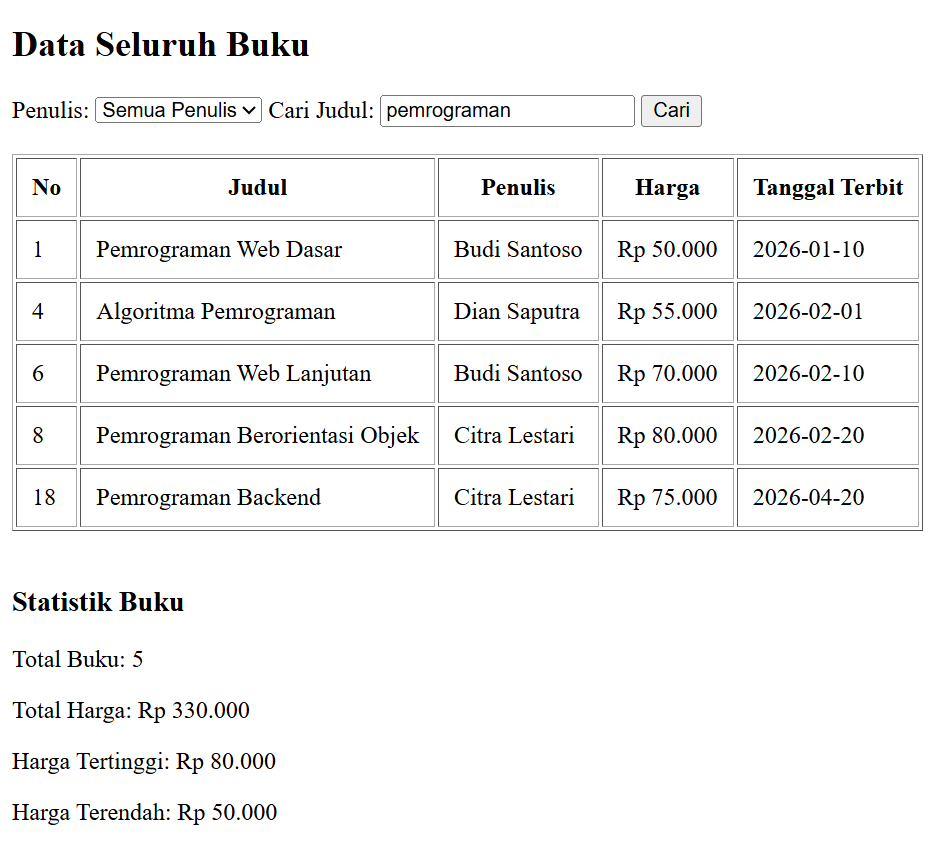
\includegraphics[width=0.96\textwidth,height=0.58\textheight,keepaspectratio]{Screenshot/buku-search-berhasil.png}
  \caption{Hasil pencarian judul buku dengan kata kunci ``pemrograman''.}
\end{figure}
Kata kunci yang tidak cocok menghasilkan pesan bahwa buku tidak ditemukan. Statistik pada halaman ini dihitung dari hasil pencarian yang sedang ditampilkan, sehingga nilainya nol saat tidak ada hasil.
\begin{figure}[H]
  \centering
  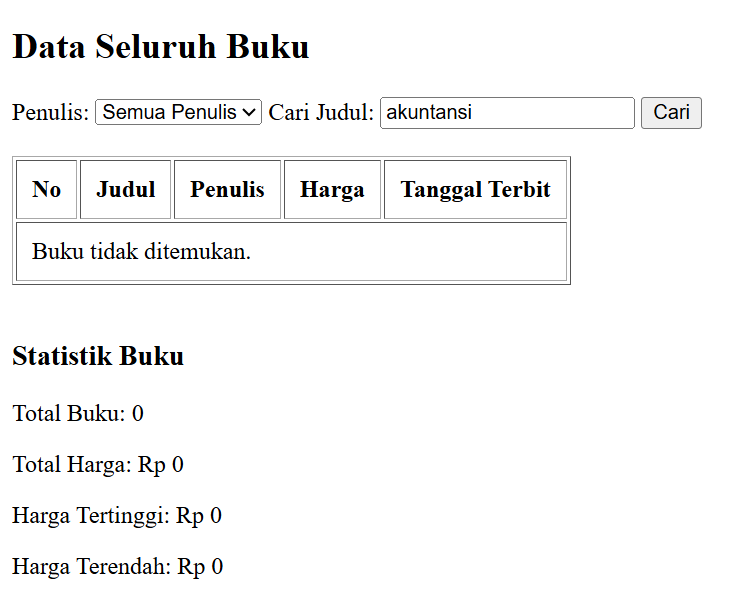
\includegraphics[width=0.96\textwidth,height=0.58\textheight,keepaspectratio]{Screenshot/buku-search-gagal.png}
  \caption{Pesan ketika pencarian judul buku tidak menemukan hasil.}
\end{figure}

\section{Proyek Trail Run}
Proyek Trail Run menampilkan data event dengan atribut nama event, penyelenggara, tipe event, tanggal mulai, dan tanggal selesai. Seeder berisi 20 event. Halaman dapat dibuka melalui URL \texttt{/event}.

\subsection{Struktur Model dan Seeder Event}
Model \texttt{Event} menghubungkan aplikasi dengan tabel \texttt{events}. Seeder mendefinisikan 20 event yang terdiri atas tipe Run, Trail Run, dan Challenge.
\lstinputlisting[language=PHP,caption={Model Event}]{Kode/Event.php}
\lstinputlisting[language=PHP,caption={Seeder berisi 20 data event}]{Kode/EventSeeder.php}

\subsection{Controller Event}
Controller mengambil lima event dengan tanggal mulai terbaru, menerapkan filter tipe event dan pencarian nama event. Statistik menampilkan jumlah seluruh event dan jumlah event berdasarkan tipe.
\lstinputlisting[language=PHP,caption={Logika daftar, filter, pencarian, dan statistik event}]{Kode/EventController.php}

\subsection{Route dan View Event}
Route halaman event menghubungkan URL \texttt{/event} dengan method \texttt{index()} pada controller event. View menampilkan jadwal, pilihan tipe, form pencarian, pesan hasil kosong, dan statistik.
\begin{lstlisting}[language=PHP,caption={Route halaman event}]
Route::get('/event', [EventController::class, 'index']);
\end{lstlisting}
\lstinputlisting[caption={View halaman Data Event Trail Run}]{Kode/event.blade.php}

\subsection{Hasil Halaman Trail Run}
Tampilan awal menunjukkan lima event terbaru dan 20 event pada tabel utama. Statistik keseluruhan terdiri atas 7 event Run, 7 event Trail Run, dan 6 event Challenge.
\begin{figure}[H]
  \centering
  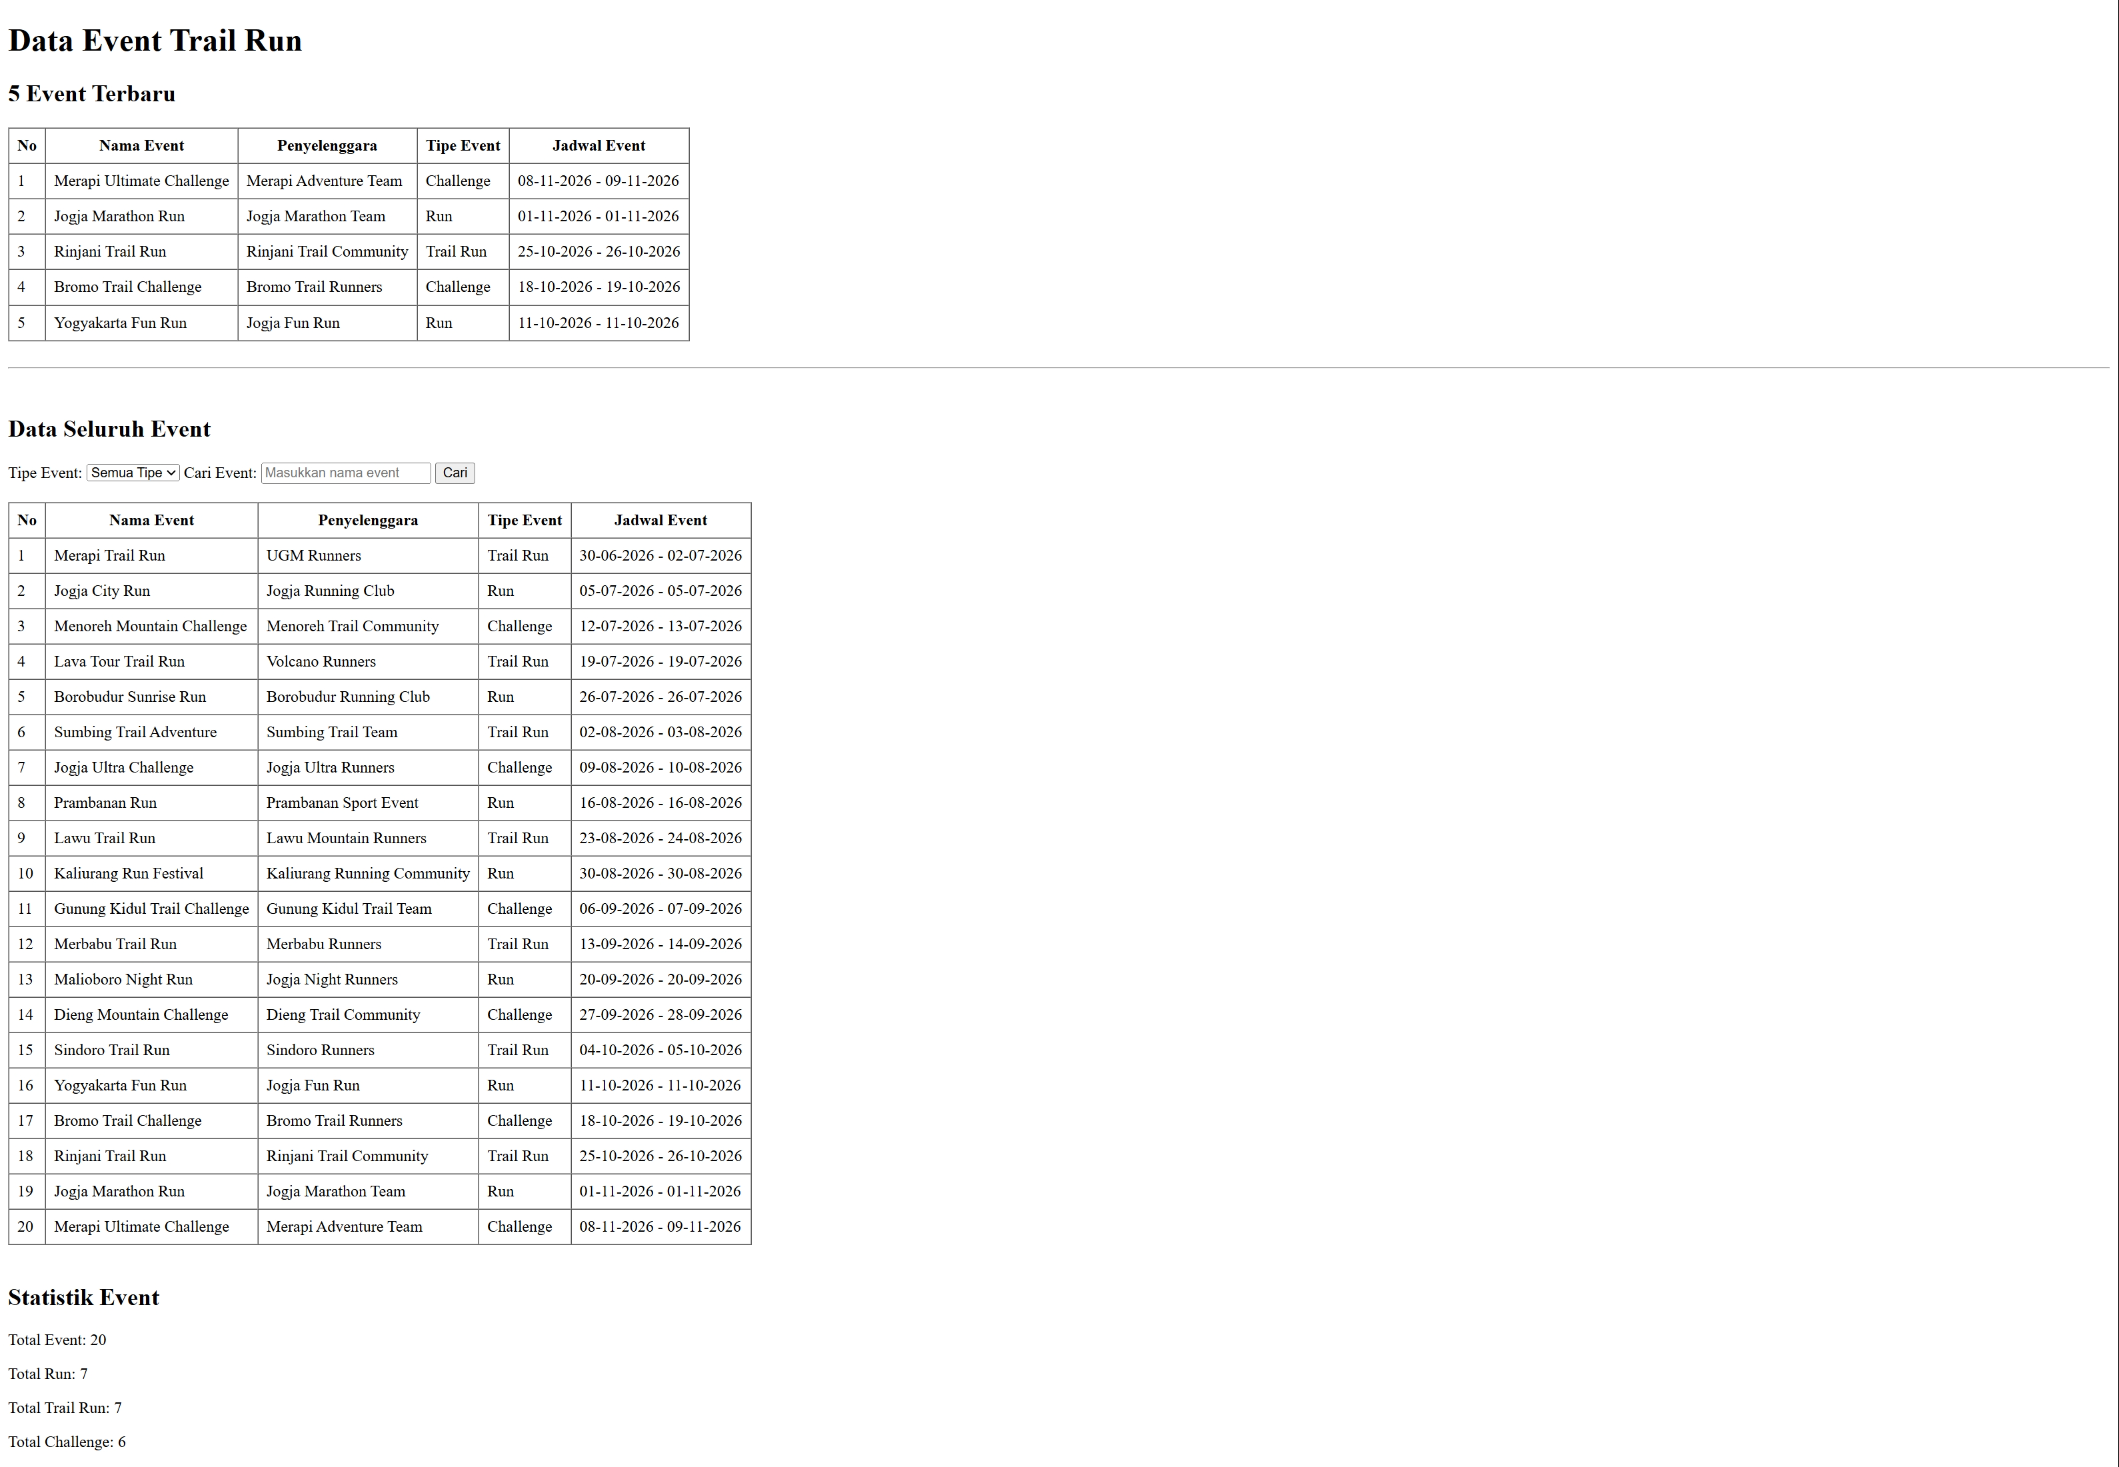
\includegraphics[height=0.72\textheight,keepaspectratio,trim=0bp 0bp 1300bp 0bp,clip]{Screenshot/trailrun-full-page.png}
  \caption{Tampilan lengkap halaman Event Trail Run, termasuk daftar event dan statistik.}
\end{figure}

\subsection{Filter Tipe Event}
Pilihan tipe event menyaring daftar sesuai tipe yang dipilih. Screenshot berikut menunjukkan data setelah filter Run diterapkan.
\begin{figure}[H]
  \centering
  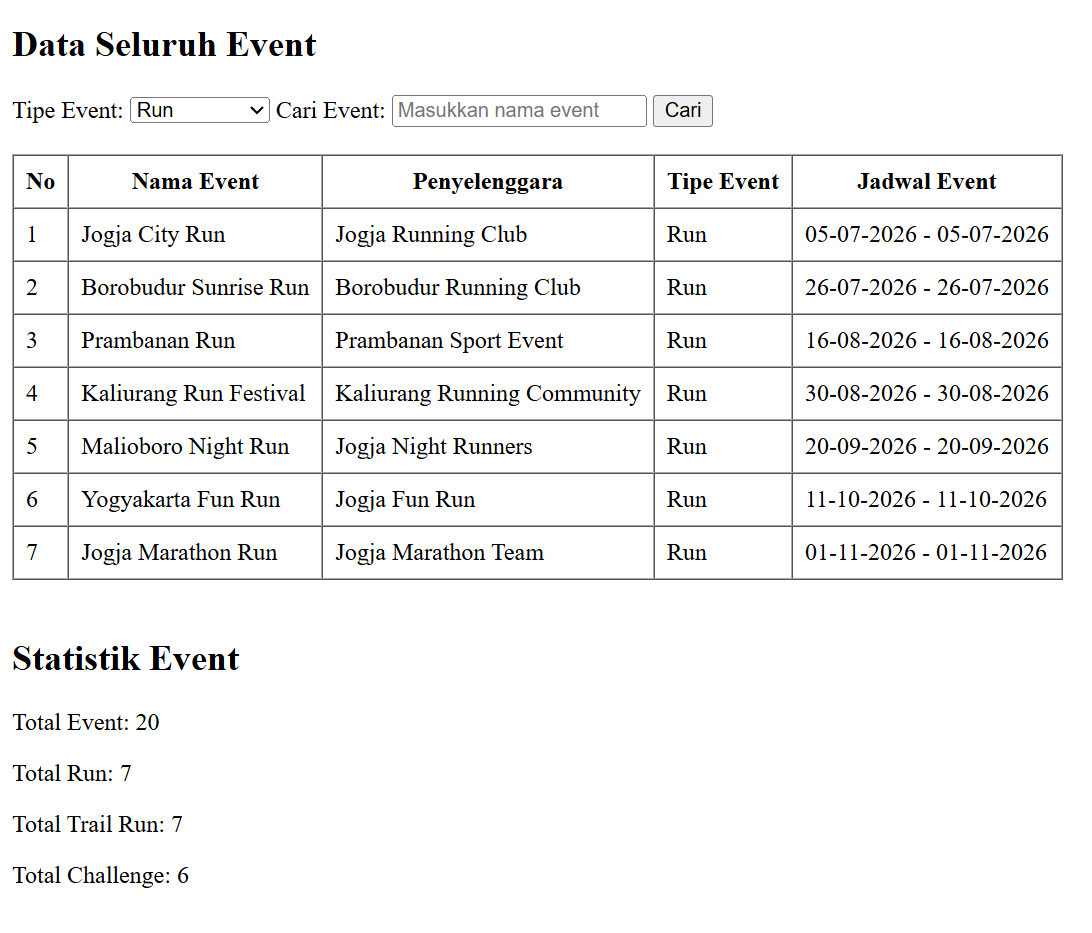
\includegraphics[width=0.96\textwidth,height=0.58\textheight,keepaspectratio]{Screenshot/trailrun-filter.png}
  \caption{Hasil filter event dengan tipe Run.}
\end{figure}

\subsection{Pencarian Nama Event}
Pencarian dengan kata kunci \texttt{joga} menghasilkan tiga event yang namanya cocok. Kata kunci tetap terlihat pada kolom pencarian setelah hasil ditampilkan.
\begin{figure}[H]
  \centering
  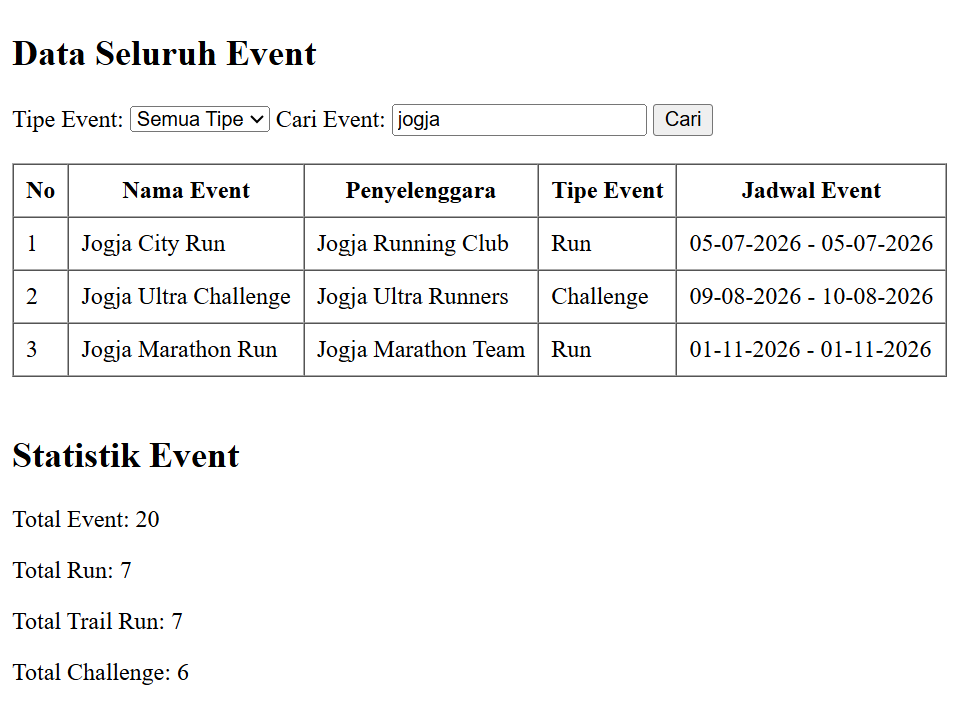
\includegraphics[width=0.96\textwidth,height=0.58\textheight,keepaspectratio]{Screenshot/trailrun-search-berhasil.png}
  \caption{Hasil pencarian event dengan kata kunci ``joga''.}
\end{figure}
Pencarian tanpa hasil menampilkan pesan \texttt{Event tidak ditemukan}. Statistik event tetap memperlihatkan jumlah keseluruhan data.
\begin{figure}[H]
  \centering
  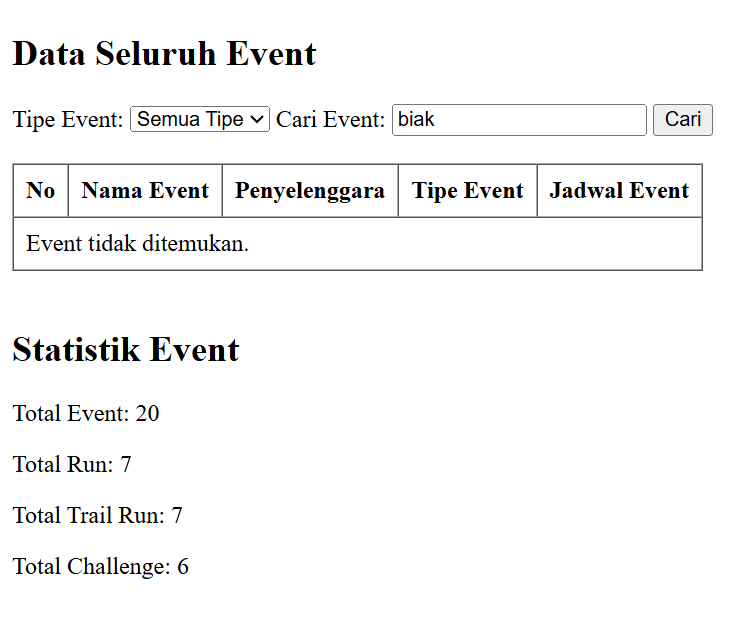
\includegraphics[width=0.96\textwidth,height=0.58\textheight,keepaspectratio]{Screenshot/trailrun-search-gagal.png}
  \caption{Pesan ketika pencarian nama event tidak menemukan hasil.}
\end{figure}

\chapter{Kesimpulan}
\section{Kesimpulan}
\begin{enumerate}
  \item Seeder pada proyek Buku dan Trail Run digunakan untuk menyiapkan masing-masing 20 data awal.
  \item Controller dan model mengolah data untuk menampilkan lima data terbaru, filter, pencarian, serta statistik.
  \item View Blade menampilkan data dalam tabel dan mempertahankan kata kunci pencarian setelah form dikirim.
  \item Kedua proyek memberikan pesan saat pencarian tidak menemukan data. Statistik Buku mengikuti hasil yang sedang ditampilkan, sedangkan statistik Trail Run merangkum seluruh data event.
\end{enumerate}

\clearpage
\phantomsection
\addcontentsline{toc}{chapter}{Daftar Pustaka}
\renewcommand{\bibname}{Daftar Pustaka}
\begin{thebibliography}{99}
\bibitem{laravel-seeding} Laravel. (2024). \textit{Database: Seeding -- Laravel 11.x Documentation}. Diakses dari \url{https://laravel.com/docs/11.x/seeding}.
\bibitem{laravel-routing} Laravel. (2024). \textit{Routing -- Laravel 11.x Documentation}. Diakses dari \url{https://laravel.com/docs/11.x/routing}.
\bibitem{laravel-blade} Laravel. (2024). \textit{Blade Templates -- Laravel 11.x Documentation}. Diakses dari \url{https://laravel.com/docs/11.x/blade}.
\bibitem{laravel-query} Laravel. (2024). \textit{Database: Query Builder -- Laravel 11.x Documentation}. Diakses dari \url{https://laravel.com/docs/11.x/queries}.
\end{thebibliography}
\end{document}
